\documentclass[UTF8]{ctexart}

\usepackage{subfiles}  

%下面的语句, 引入你的头部设置文件
\usepackage{C:/phpStorm_proj/02_myself_ID_EGO/+100_latex_all_math_sel/myPreamble} 
%必须是绝对路径,才能让各个tex在单独编译时使用到

\title{文件名}


%---------------------------------


\begin{document}
	\tableofcontents % 生成目录
	\date{} % 若不写这句, 则默认也会渲染出日期, 所以我们要手动赋空值
	\maketitle  %这行代码, 让你前面的 title, author, date生效
	
	\part{分位数 Quantile}
	
		
	\section{``分位数"的定义} 	
	``某"分位数, 指的就是连续数据的"概率函数 f(x)"的x轴上的一个点,这个点对应着``其左侧的曲线下的面积"(即概率值)=``某". \\
	
	比如下图, \textbf{$x_p$ 就是"p分位数". 意思是: 在$x_p$这个点处, 该点左侧的曲线下的面积值=p . 即 $P{X \leq x_p} = p$.} \\	
	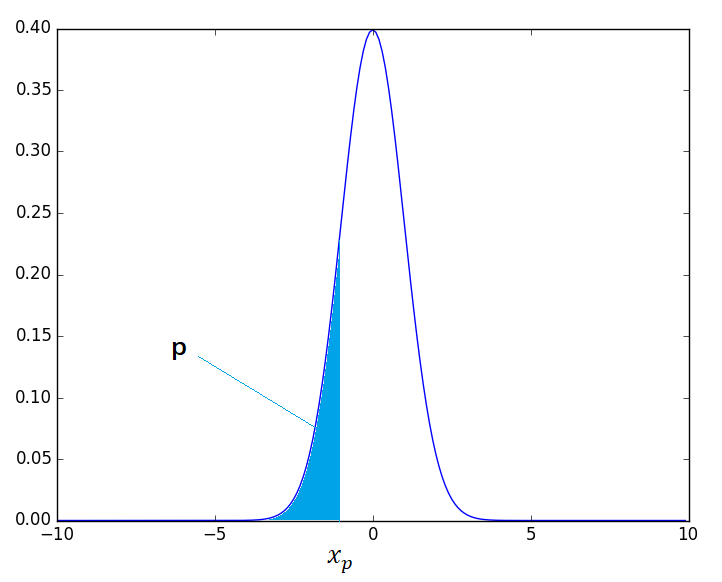
\includegraphics[width=0.5\textwidth]{/0216.png} 
	
	
	
	\section{上侧$\alpha$分位数$u_{\alpha}$ : 就是x轴上的一个点. 该点右侧曲线下的面积=$\alpha$}
	\textbf{X 是个正态分布, 即 $X \sim N(0,1)$.  我们规定 $\alpha$的取值范围是 $(0< \alpha <1)$, 即 $\alpha$点只能处在x=(0,1)的区间上. 然后, 你去x轴上找一个点的位置 $u_α$, 要使得 $P\{X>u_{\alpha}\}\text{的概率}=\alpha$, 则, 这个  $u_{\alpha}$点, 就叫做``上$\alpha$分位数".} \\	
	
	即 : $ \boxed{
		P\{X>\underset{\text{上}\alpha \text{分位数}}{\underbrace{u_{\alpha}}}\}=\underset{\text{概率值}}{\underbrace{\alpha }}\\
	}$ \\
	
	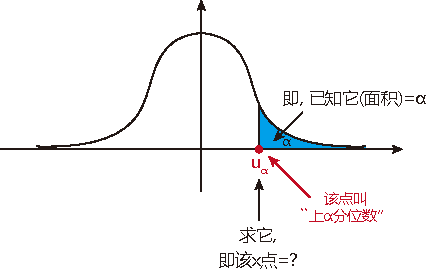
\includegraphics[width=0.55\textwidth]{/0220.pdf} \\
	
	\begin{myEnvSample}
	比如, 已知概率值 $\alpha=0.05$, 我们要找x轴上的这个点 $u_{0.05}$ 的具体值是几? \\
	即, 已知 $	P\{X>\underset{\text{上0.05分位数}}{\underbrace{u_{0.05}}}\}=\underset{\text{概率值}\alpha =0.05}{\underbrace{0.05}}$, 求$u_{0.05}=?$ \\
	
	
	从geogebra中的计算可知, $u_{0.05}=1.645$ \\	
	
	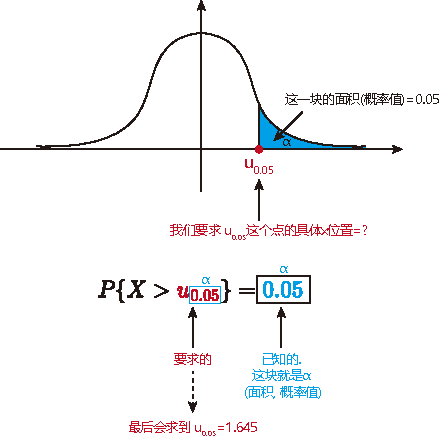
\includegraphics[width=0.6\textwidth]{/0219.pdf} \\
		
	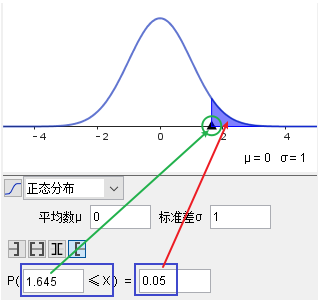
\includegraphics[width=0.5\textwidth]{/0218.png} 	
	\end{myEnvSample}
	
	\textbf{所以我们现在就知道了, 上$\alpha$分位数, 它其实就是 x轴上的一个点, 只不过它的变量名写作了: $u_{\text{右侧曲线下的面积}}$.} \\
	
	
	\begin{myEnvSample}
又比如: \\
$P\{X>\underset{\text{要求的}.=1.96}{\underbrace{u_{0.025}}}\}=\underset{\text{已知的}}{\underbrace{0.025}}$ \\
	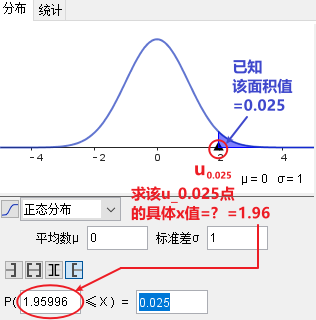
\includegraphics[width=0.55\textwidth]{/0221.png} 
	\end{myEnvSample}
	
	
	
\end{document}